%==============================================================================
%  Wi-Fi CSI-Based Device-Free Motion Detection
%  Final project report
%
%  COMPILING
%  ---------
%  Overleaf: upload this file, set the compiler to pdfLaTeX (Menu > Compiler),
%  and compile twice so the table of contents and cross-references settle.
%  Locally:  pdflatex csi_final_report.tex   (run it twice)
%
%  Every package used here ships with a standard TeX Live / Overleaf install.
%  There are NO external image files and NO shell-escape requirements: the two
%  charts and the architecture diagram are drawn from the real numbers with
%  pgfplots and TikZ, so the document is self-contained and cannot break
%  because an asset is missing.
%==============================================================================

\documentclass[11pt,a4paper]{article}

%------------------------------------------------------------------ packages --
\usepackage[utf8]{inputenc}          % source encoding (harmless on modern TeX)
\usepackage[T1]{fontenc}             % proper hyphenation and copy-pasteable text
\usepackage[english]{babel}
\usepackage[margin=2.5cm]{geometry}  % page margins

\usepackage{amsmath}                 % align, equation environments
\usepackage{amssymb}
\usepackage{graphicx}                % \includegraphics (for optional screenshots)
\usepackage{booktabs}                % \toprule \midrule \bottomrule
\usepackage{longtable}               % tables that break across pages
\usepackage{array}
\usepackage{multirow}
\usepackage{tabularx}
\usepackage{caption}
\usepackage{float}                   % the [H] float placement specifier
\usepackage{enumitem}                % compact lists
\usepackage{xcolor}
\usepackage{listings}                % code and command listings
\usepackage{fancyhdr}                % running headers
\usepackage{titlesec}

\usepackage{tikz}
\usetikzlibrary{arrows.meta, positioning, shapes.geometric, fit, backgrounds}
\usepackage{pgfplots}
\pgfplotsset{compat=1.18}            % pin behaviour so the charts render the same

\usepackage[colorlinks=true,
            linkcolor=blue!45!black,
            urlcolor=blue!45!black,
            citecolor=blue!45!black]{hyperref}
\hypersetup{
  pdftitle={Wi-Fi CSI-Based Device-Free Motion Detection},
  pdfauthor={Ilyas},
  pdfsubject={Wi-Fi sensing, embedded machine learning},
  pdfkeywords={CSI, Wi-Fi sensing, ESP32-S3, Random Forest, device-free sensing}
}

%------------------------------------------------------------------- styling --
\definecolor{codebg}{RGB}{246,246,244}
\definecolor{accent}{RGB}{15,98,208}
\definecolor{good}{RGB}{21,127,61}
\definecolor{bad}{RGB}{194,53,47}
\definecolor{warn}{RGB}{162,104,11}
\definecolor{rulegrey}{RGB}{120,120,120}

\lstdefinestyle{codestyle}{
  backgroundcolor=\color{codebg},
  basicstyle=\ttfamily\footnotesize,
  breaklines=true,
  breakatwhitespace=false,
  frame=single,
  framerule=0.3pt,
  rulecolor=\color{rulegrey},
  xleftmargin=6pt,
  xrightmargin=2pt,
  aboveskip=10pt,
  belowskip=6pt,
  keywordstyle=\color{accent}\bfseries,
  commentstyle=\color{good}\itshape,
  stringstyle=\color{warn},
  showstringspaces=false,
  tabsize=2,
  captionpos=b,
}
\lstset{style=codestyle}

\pagestyle{fancy}
\fancyhf{}
\fancyhead[L]{\small\itshape Wi-Fi CSI-Based Device-Free Motion Detection}
\fancyhead[R]{\small\thepage}
\renewcommand{\headrulewidth}{0.3pt}

% Shorthands. Underscores must be escaped in text mode, so folder and symbol
% names go through these rather than being typed inline every time.
\newcommand{\code}[1]{\texttt{\small #1}}
\newcommand{\sessA}{\code{part\_1\_data}}
\newcommand{\sessNames}{\code{part\_1\_data}\,\dots\,\code{part\_8\_data}}
\newcommand{\roomA}{\code{room2\_part\_1\_data}}
\newcommand{\roomB}{\code{room2\_part\_2\_data}}
\newcommand{\keyfinding}[1]{%
  \begin{center}\fbox{\begin{minipage}{0.93\linewidth}\vspace{2pt}#1\vspace{2pt}\end{minipage}}\end{center}}

%==============================================================================
\begin{document}
%==============================================================================

%------------------------------------------------------------------ title ----
\begin{titlepage}
\centering
\vspace*{2.2cm}

{\Large\scshape Project Report}\\[0.4cm]
\rule{\linewidth}{0.4pt}\\[0.7cm]

{\huge\bfseries Wi-Fi CSI-Based Device-Free\\[0.25cm] Motion Detection}\\[0.7cm]

{\large Design, Data Collection, Model Validation, Live Inference\\
and Standalone Deployment on an ESP32-S3}\\[0.5cm]

\rule{\linewidth}{0.4pt}\\[1.6cm]

{\large\textbf{Ilyas}}\\[0.3cm]
% ---- EDIT THESE THREE LINES -------------------------------------------------
{\normalsize Department / Programme}\\[0.15cm]
{\normalsize Institution}\\[0.15cm]
{\normalsize Supervisor: \textit{name}}\\[1.6cm]
% -----------------------------------------------------------------------------

{\large \today}\\[2.0cm]

\begin{minipage}{0.86\linewidth}\small
\textit{Source code, datasets and the full development history are available at}\\
\url{https://github.com/IALR/csi-motion-detection}
\end{minipage}

\vfill
\end{titlepage}

%--------------------------------------------------------------- abstract ----
\begin{abstract}
\noindent
This report describes the design, implementation and evaluation of a
device-free motion detection system built on Wi-Fi Channel State Information
(CSI). A person moving through a room perturbs the multipath propagation
between a transmitter and a receiver; because every Wi-Fi receiver already
estimates the channel in order to decode packets, that perturbation can be
harvested as a by-product of ordinary communication, with no camera, no
wearable device and no dedicated sensing hardware.

The system uses one or two ESP32-S3 boards as receivers, streaming
per-subcarrier amplitude at approximately ten frames per second to a host that
extracts a 266-dimensional, calibration-relative feature vector per
0.75-second window and classifies it with a Random Forest. The classifier
reaches \textbf{94.25\,\% leave-one-session-out accuracy} across ten recording
sessions in two rooms.

Two findings are emphasised. First, a single accuracy figure is an inadequate
description of this class of system: performance is strongly
environment-dependent, and the empty-room radio noise floor varied by a factor
of roughly nine across the project's own recordings, with accuracy ranging from
84.67\,\% to 98.69\,\% between held-out sessions. The system therefore measures
and reports which regime it is operating in rather than degrading silently.
Second, the same model was exported to C and verified to run on the
microcontroller itself with exact parity against the host implementation
(3302/3302 windows), allowing the board to perform detection and serve its own
web dashboard with no computer attached.

The report also documents negative results, refuted hypotheses and recurring
failure modes, on the argument that these are the most transferable part of an
engineering project.
\end{abstract}

\clearpage
\tableofcontents
\clearpage

%==============================================================================
\section{Introduction}
%==============================================================================

\subsection{Motivation}

Conventional occupancy sensing relies on cameras, passive infrared detectors,
pressure mats or devices carried by the occupant. Each carries a cost: cameras
raise obvious privacy objections and fail in darkness, infrared detectors are
line-of-sight and respond to thermal sources rather than to people
specifically, and wearable approaches only work for cooperating subjects who
remember to carry the device.

Wi-Fi sensing offers a different trade. Radio waves at 2.4\,GHz pass through
furniture and interior walls, propagate in darkness, and --- critically --- are
already present in almost every indoor environment. A human body is largely
water and interacts strongly with radiation at this frequency, so a person
moving through a room continuously alters the set of paths by which a signal
reaches a receiver. If that alteration can be measured, occupancy can be
inferred without instrumenting the person at all. This is referred to as
\emph{device-free} sensing.

The measurement itself requires no new hardware. Every Wi-Fi receiver must
estimate how the channel distorted an incoming signal in order to decode it,
and on some chipsets that estimate --- the Channel State Information --- can be
read out. This project treats CSI as a sensing modality rather than as an
internal implementation detail of the radio.

\subsection{Problem statement}

The system answers one question, continuously and in real time:

\keyfinding{\centering\textbf{Is the monitored room empty, or is someone moving in it?}}

\noindent
This is a binary classification problem over short time windows. The two
classes are labelled \code{0} (EMPTY) and \code{2} (MOVING) throughout the
codebase and this report.

\subsection{Scope and explicit non-goals}

Stating the boundaries early prevents the results from being read as claims the
evidence does not support. The system does \emph{not}:

\begin{itemize}[leftmargin=1.4em, itemsep=2pt]
  \item \textbf{localise} a person in coordinates. True positional estimation
        requires signal \emph{phase} and multiple \emph{synchronised} antennas
        per receiver; this system is amplitude-only and its two boards share no
        clock. Section~\ref{sec:limitations} develops this point.
  \item \textbf{count or identify} people. Two occupants read the same as one.
  \item \textbf{detect a motionless person.} A person sitting still is
        classified as EMPTY. This is a motion detector, not a presence
        detector, and the distinction is material.
  \item \textbf{constitute a security product.} It has no tamper detection, no
        redundancy and no fail-safe behaviour.
\end{itemize}

\subsection{Contributions}

The substantive contributions of the work are:

\begin{enumerate}[leftmargin=1.6em, itemsep=3pt]
  \item A \textbf{data collection protocol} that resolves the practical
        contradiction in labelling this task: the operator must be absent to
        record ``empty'' and present to record ``moving''
        (Section~\ref{sec:data}).
  \item A \textbf{calibration-relative feature formulation} that expresses each
        window relative to a recent confirmed-empty baseline, so that the model
        learns disturbance rather than the static signature of one room
        (Section~\ref{sec:features}).
  \item A \textbf{session-level validation methodology} and an argument for why
        the more common random split would substantially overstate performance
        for this data (Section~\ref{sec:validation}).
  \item A \textbf{scale-free empty-room noise floor metric}, together with
        thresholds derived from the project's own recordings, which quantifies
        how favourable the current environment is and is reported live
        (Section~\ref{sec:noise}).
  \item A \textbf{verified embedded port}: the identical trained forest exported
        to C and shown to reproduce the host implementation exactly, enabling
        laptop-free operation (Section~\ref{sec:embedded}).
  \item A record of \textbf{negative results and recurring failure modes}
        (Sections~\ref{sec:recurring} and \ref{sec:negative}).
\end{enumerate}

%==============================================================================
\section{Background}
%==============================================================================

\subsection{Channel State Information}

Modern Wi-Fi uses Orthogonal Frequency-Division Multiplexing (OFDM), which
divides the channel into a set of narrow, closely spaced \emph{subcarriers}
transmitted in parallel. Because each subcarrier occupies a different
frequency, each experiences the propagation environment slightly differently.
To decode a packet the receiver estimates, for every subcarrier, the complex
gain the channel applied to it. That collection of per-subcarrier complex
estimates is the Channel State Information.

For a transmitted symbol $X_k$ on subcarrier $k$ and a received symbol $Y_k$,
the channel estimate $H_k$ satisfies
\begin{equation}
  Y_k = H_k X_k + N_k ,
\end{equation}
where $N_k$ is noise. $H_k$ is complex, carrying both an amplitude and a phase.
The ESP32 firmware used here reports $H_k$ as signed 8-bit in-phase and
quadrature components, from which amplitude is computed as
\begin{equation}
  a_k = \sqrt{\Re(H_k)^2 + \Im(H_k)^2}.
  \label{eq:amp}
\end{equation}

\subsection{Why motion perturbs CSI}

A signal does not reach the receiver by one path. It arrives by the direct
line-of-sight path and by many reflected paths --- off walls, floor, ceiling
and furniture. These copies arrive with different delays and therefore
different phase rotations, and they sum at the antenna. Because the phase
rotation of a given path depends on its length \emph{in wavelengths}, and the
wavelength differs slightly between subcarriers, the sum is different at every
subcarrier. This is why the amplitudes $a_k$ are not flat across the band but
form a structured, room-specific profile.

A stationary room produces a nearly constant profile. Introducing a person adds
new reflecting surfaces and blocks existing paths; moving that person changes
the corresponding path lengths continuously, so the profile fluctuates. The
detection problem is therefore to distinguish \emph{structured fluctuation
caused by a moving body} from the residual fluctuation of an empty room. As
Section~\ref{sec:noise} shows, the difficulty of that discrimination depends
almost entirely on how large the residual fluctuation is.

\subsection{Amplitude-only sensing}

The firmware computes Equation~\ref{eq:amp} and \textbf{discards phase} before
any data leaves the board. This was a deliberate scope decision rather than an
oversight, and it has two consequences that should be stated plainly:

\begin{itemize}[leftmargin=1.4em, itemsep=2pt]
  \item Raw CSI phase on commodity hardware is corrupted by carrier frequency
        offset, sampling time offset and random packet detection delay. Using it
        requires a sanitisation step that this project did not undertake.
  \item Without phase, techniques that estimate angle-of-arrival or
        time-of-flight are unavailable. This is the technical reason
        localisation is out of scope.
\end{itemize}

\subsection{Channel width and subcarrier count}
\label{sec:width}

One property of the physical layer propagates all the way up into the machine
learning pipeline and deserves emphasis, because it caused repeated failures
during development:

\keyfinding{The number of CSI subcarriers is fixed by the channel width.
A \textbf{20\,MHz} channel yields \textbf{128} subcarriers; a \textbf{40\,MHz}
channel yields \textbf{192}. The trained model expects exactly 128, so an
access point that renegotiates its channel width silently invalidates every
feature vector the system produces.}

\noindent
Approximately 20 of the 128 subcarriers are structurally dead --- OFDM guard
bands and the DC null --- and report an amplitude of exactly zero at all times.
Section~\ref{sec:deadsub} shows that failing to account for these caused a
serious and initially invisible defect in the feature extraction.

%==============================================================================
\section{System Architecture}
%==============================================================================

\subsection{Overview}

Figure~\ref{fig:arch} shows the signal path. The essential point is that CSI
\emph{only exists when a packet is received}. An idle station receives almost
nothing and therefore produces almost no CSI. The firmware manufactures a
steady measurement stream by transmitting an ICMP echo request to the access
point every 100\,ms and taking a CSI sample from each reply, giving the
approximately 10\,Hz frame rate used throughout.

\begin{figure}[H]
\centering
\begin{tikzpicture}[
  font=\small,
  node distance=8mm,
  box/.style={draw, rounded corners=2pt, align=center, minimum height=8mm,
              inner sep=4pt, fill=codebg},
  proc/.style={box, fill=blue!6},
  out/.style={box, fill=green!7},
  arr/.style={-{Latex[length=2mm]}, thick}
]

\node[box] (ap)   {Access point\\(20\,MHz)};
\node[box, below=14mm of ap] (esp) {ESP32-S3\\receiver};
\node[proc, right=22mm of esp] (parse) {Parse\\\code{CSI\_AMP} line};
\node[proc, right=14mm of parse] (win)  {Window\\0.75\,s / 8 frames};
\node[proc, below=10mm of win] (feat) {Calibrated features\\(266-dim)};
\node[proc, left=14mm of feat] (base) {Baseline\\(10\,s empty)};
\node[proc, below=10mm of feat] (rf)  {Random Forest\\200 trees};
\node[out, below left=10mm and 2mm of rf] (smooth) {Smoothing\\majority of 5};
\node[out, right=16mm of smooth] (fuse) {OR fusion\\(2 nodes)};

\draw[arr] (ap) -- node[right, font=\scriptsize] {ping reply, 10\,Hz} (esp);
\draw[arr] (esp) -- node[above, font=\scriptsize] {USB serial} (parse);
\draw[arr] (parse) -- (win);
\draw[arr] (win) -- (feat);
\draw[arr] (base) -- (feat);
\draw[arr] (feat) -- (rf);
\draw[arr] (rf) -- (smooth);
\draw[arr] (smooth) -- (fuse);

\node[draw, dashed, rounded corners, inner sep=6pt, fit=(parse)(win)(feat)(base)(rf)(smooth)(fuse),
      label={[font=\scriptsize\itshape]above right:host pipeline, or on-device in standalone mode}] {};
\end{tikzpicture}
\caption{Signal path from access point to classified state. In standalone mode
the entire dashed region runs on the ESP32-S3 itself.}
\label{fig:arch}
\end{figure}

\subsection{Hardware and firmware}

\begin{table}[H]
\centering
\caption{Platform configuration.}
\begin{tabular}{@{}ll@{}}
\toprule
\textbf{Item} & \textbf{Value} \\
\midrule
Microcontroller        & ESP32-S3 \\
Framework              & ESP-IDF v6.0.2 \\
Flash                  & 16\,MB, custom partition table with a 4\,MB application slot \\
Firmware image size    & 1.27\,MB (approximately 68\,\% of the slot free) \\
Console baud rate      & 115200 \\
CSI trigger            & ICMP echo to the gateway every 100\,ms \\
Channel width          & pinned to 20\,MHz by the station \\
Frame rate             & approximately 10 frames per second \\
Subcarriers reported   & 128 (about 108 carrying signal) \\
\bottomrule
\end{tabular}
\end{table}

\noindent
The firmware performs four tasks: it joins the configured network, pins its own
link to 20\,MHz, generates the ping traffic that produces CSI, and formats each
frame as a single line on the serial console:

\begin{lstlisting}[caption={Serial line format emitted by the firmware.}]
CSI_AMP,<timestamp_us>,<label>,<num_subcarriers>,<rssi>,<amp0>,<amp1>,...
\end{lstlisting}

\noindent
Two design details are worth noting. CSI frames are filtered by the access
point's BSSID, so only frames from the network of interest are retained.
And the CSI callback, which runs in the Wi-Fi task, does nothing but copy the
buffer into a queue; all formatting and serial output happen in a separate
printer task, so a slow console cannot stall the radio.

\subsection{Deployment modes}

\begin{table}[H]
\centering
\caption{The three supported deployments.}
\begin{tabularx}{\linewidth}{@{}lX@{}}
\toprule
\textbf{Mode} & \textbf{Description} \\
\midrule
Single node + host & One board streams over USB; a Python process classifies and
serves a dashboard over WebSocket. \\
Two nodes + host   & Two fully independent pipelines --- separate ports,
baselines, windows and smoothers --- combined with OR logic. \\
Standalone         & The board runs the identical exported model on-device and
serves the same dashboard itself over HTTP and WebSocket. No computer is
involved. Single-node only. \\
\bottomrule
\end{tabularx}
\end{table}

%==============================================================================
\section{Data Collection Methodology}
\label{sec:data}
%==============================================================================

\subsection{The labelling contradiction}

Supervised learning requires labelled examples of both classes, but the two
classes here impose contradictory requirements on the operator: recording
``empty'' requires that nobody is in the room, while recording ``moving''
requires that somebody is. A single person collecting data alone cannot
simply annotate a continuous recording, because the act of entering the room to
start or stop the recording contaminates precisely the data being collected.

CSI is sensitive enough that this is not a hypothetical concern. During
development, one recording session was discarded after analysis showed that a
person lingering near a doorway during the supposed empty period had produced
enough disturbance to make the empty class overlap the moving class.

\subsection{The auto-cycling protocol}

The collector resolves this by making the empty blocks automatic and the moving
blocks manual:

\begin{enumerate}[leftmargin=1.6em, itemsep=2pt]
  \item A five-second countdown instructs the operator to leave the room.
        Frames captured during the countdown are written with
        \code{settling=1} and are discarded at training time.
  \item Sixty seconds of EMPTY (label \code{0}) are recorded automatically.
  \item The system waits indefinitely. Nothing is recorded while the operator
        returns.
  \item On a keypress, sixty seconds of MOVING (label \code{2}) are recorded.
  \item The cycle repeats until stopped.
\end{enumerate}

\noindent
The \code{settling} column is a deliberate design choice: rather than trying to
guess when the operator has left, the ambiguous frames are captured, flagged,
and removed downstream. This makes the contamination boundary explicit and
auditable instead of implicit.

\subsection{Dataset}

\begin{table}[H]
\centering
\caption{Recording sessions. All sessions are 128 subcarriers at approximately
10\,Hz, and all are included in the training set of the deployed model.}
\label{tab:dataset}
\begin{tabular}{@{}llrrl@{}}
\toprule
\textbf{Session} & \textbf{Room} & \textbf{Frames} & \textbf{Empty / Moving} & \textbf{Notes} \\
\midrule
\code{part\_1\_data} & 1 & 1276 & 676 / 600 & first session \\
\code{part\_2\_data} & 1 & 2656 & 1456 / 1200 & \\
\code{part\_3\_data} & 1 & 2802 & 1602 / 1200 & \\
\code{part\_4\_data} & 1 & 2648 & 1448 / 1200 & original held-out test \\
\code{part\_5\_data} & 1 & 2637 & 1437 / 1200 & air conditioning switched on mid-session \\
\code{part\_6\_data} & 1 & 2605 & 1405 / 1200 & continuous drift; noisy \\
\code{part\_7\_data} & 1 & 2608 & 1408 / 1200 & less vigorous movement \\
\code{part\_8\_data} & 1 & 2619 & 1419 / 1200 & window deliberately opened; noisy \\
\code{room2\_part\_1\_data} & 2 & 5019 & 2618 / 2401 & cross-room test \\
\code{room2\_part\_2\_data} & 2 & 3767 & 1967 / 1800 & folded into training \\
\midrule
\textbf{Total} & & \textbf{28\,637} & & approximately 48 minutes \\
\bottomrule
\end{tabular}
\end{table}

\noindent
After discarding settling frames and forming non-overlapping windows, the
dataset yields \textbf{3302 windows}: 1654 empty and 1648 moving. The classes
are therefore almost exactly balanced, which is why plain accuracy is a
defensible headline metric for this problem.

\subsection{Rejected recordings}

Four recordings were made and deliberately discarded, and it is more honest to
report them than to present only the surviving data:

\begin{itemize}[leftmargin=1.4em, itemsep=2pt]
  \item Two attempts at session 4 --- one with a contaminated empty block, one
        in which the hardware was inadvertently repositioned partway through.
  \item Two attempts at session 5 --- one recorded at 192 subcarriers after the
        access point auto-negotiated a 40\,MHz channel
        (Section~\ref{sec:width}), and one that was technically valid but
        confounded a room change with a change in movement style.
\end{itemize}

\noindent
Each re-recording reused the same folder name, so the earlier attempts were
overwritten and are not recoverable.

%==============================================================================
\section{Feature Engineering}
\label{sec:features}
%==============================================================================

\subsection{Why absolute features fail}

The first version of this system used absolute features: the mean amplitude of
each subcarrier, its standard deviation, and the raw RSSI. This performed
acceptably within a single recording and poorly across recordings, for a reason
that is clear in retrospect.

An absolute feature encodes \emph{what this room looks like right now} at least
as strongly as it encodes \emph{whether someone is moving}. The per-subcarrier
amplitude profile is a fingerprint of the room's geometry, the position of the
furniture, the temperature of the hardware and the exact placement of the
boards. If any of those change between the training recording and deployment
--- a different day, a nudged router, thermal drift --- the whole feature
vector shifts, and a model that learned absolute thresholds interprets the
shift as motion.

\subsection{Baseline-relative formulation}

The system therefore expresses every window relative to a \emph{baseline}
computed from a block of confirmed-empty frames. Let $\mathbf{a}(t) \in
\mathbb{R}^{K}$ be the amplitude vector at frame $t$ over $K=128$ subcarriers.
For a baseline block $B$ and a scoring window $W$, define per-subcarrier means
and standard deviations $\mu^{B}_k, \sigma^{B}_k, \mu^{W}_k, \sigma^{W}_k$.

The two per-subcarrier feature families are
\begin{align}
  \Delta_k &= \mu^{W}_k - \mu^{B}_k
    &&\text{(mean shift; constant offsets cancel)}\\[2pt]
  \rho_k &= \frac{\sigma^{W}_k}{\max\!\left(\sigma^{B}_k,\ \tau\right)}
    &&\text{(spread ratio; see Section~\ref{sec:deadsub} for } \tau\text{)}
\end{align}

Expressing spread as a \emph{ratio} rather than a difference has an important
consequence: an already-noisy baseline raises the threshold for what counts as
``more disturbed than usual''. The system adapts its own sensitivity to the
environment instead of comparing against a fixed threshold learned somewhere
else on some other day.

\keyfinding{This does \emph{not} rescue a room that is never quiet during
calibration itself. If a disturbance is present throughout the baseline period
it becomes the new definition of ``empty'', and motion on top of it may still
be missed. What the formulation fixes is the specific failure mode in which
everything looks like motion because the baseline moved.}

\subsection{Dead subcarriers and the variance floor}
\label{sec:deadsub}

Approximately 20 of the 128 subcarriers are structurally dead and report
amplitude exactly zero in every frame. Their baseline standard deviation
$\sigma^{B}_k$ is therefore exactly zero, and the ratio $\rho_k$ divides by it.

The consequences were severe and, importantly, invisible in aggregate accuracy
at first. A live standard deviation of 0.001 on a dead subcarrier, divided by a
baseline of 0, produces a ratio of order $10^{3}$, against approximately $1.0$
for a genuinely stable subcarrier. Aggregate features that search for the
\emph{maximum} ratio across the band were consequently hijacked by numerical
noise on dead subcarriers in nearly every window, regardless of whether anyone
was moving. Observed ratios reached approximately $10^{4}$.

The fix is a variance floor: no subcarrier's baseline standard deviation is
allowed to count as smaller than 10\,\% of the median baseline standard
deviation for that block,
\begin{equation}
  \tau = \max\!\left(0.1 \cdot \mathrm{median}_k\!\left(\sigma^{B}_k\right),\ \varepsilon\right).
\end{equation}
The same reasoning applies to the noise-floor metric of
Section~\ref{sec:noise}, whose amplitude scale averages only the active
subcarriers, since including the dead ones would deflate the scale and inflate
the ratio.

\subsection{The feature vector}

\begin{table}[H]
\centering
\caption{The 266-dimensional feature vector.}
\label{tab:features}
\begin{tabularx}{\linewidth}{@{}rlX@{}}
\toprule
\textbf{Count} & \textbf{Family} & \textbf{Interpretation} \\
\midrule
128 & \code{amp\_mean\_delta} & per-subcarrier mean shift from baseline \\
128 & \code{amp\_std\_ratio}  & per-subcarrier fluctuation relative to baseline \\
2   & motion energy mean, std ratio & whole-band frame-to-frame change \\
2   & RSSI mean delta, std ratio & overall received-level shift \\
6   & order-invariant summaries & maximum, top-$K$ mean, 90th percentile,
      fraction elevated, and two magnitude equivalents \\
\midrule
\textbf{266} & & \\
\bottomrule
\end{tabularx}
\end{table}

\subsection{Order-invariant features and cross-room transfer}

The 256 per-subcarrier features are tied to specific subcarrier
\emph{indices}. A decision tree can therefore split on ``subcarrier 43'', which
is meaningful only because that is where this particular room's multipath
happened to place a sensitive spot. A different room's geometry puts the
sensitive band somewhere else entirely, and an index-based feature has no way
to transfer that knowledge.

The final six features are deliberately \emph{order-invariant} summaries of the
same per-subcarrier arrays: the maximum ratio, the mean of the top ten, the
90th percentile, and the fraction of subcarriers whose ratio exceeds 1.5,
together with two magnitude equivalents. These answer ``is \emph{something} in
the band disturbed'' without regard to \emph{which} index is disturbed, and
should be expected to generalise across rooms better than the index-based
features, at some cost in within-room precision. Both families are retained and
the Random Forest is free to weight whichever fits.

\subsection{Per-block recalibration}

A single baseline computed once at the start of a session was tried first and
found to go stale within minutes. Real recordings exhibited both sudden shifts
--- an air conditioning unit switching on between two empty blocks --- and slow
continuous drift, plausibly thermal.

The pipeline therefore recalibrates at \emph{every} empty block: whenever the
recording re-enters an empty period, the first ten seconds of that period
become a fresh baseline, used for every window until the next empty block
begins. The effect on the affected session was decisive.

\keyfinding{\code{part\_5\_data}, the session in which air conditioning was
switched on partway through, scored \textbf{75\,\%} held out under a
single-baseline pipeline and \textbf{99.17\,\%} after per-block recalibration
was introduced. No change was made to the model, the features or the data.}

%==============================================================================
\section{Model Selection}
%==============================================================================

The deployed classifier is a Random Forest of 200 trees with unlimited depth
and a fixed random seed. Rather than asserting that choice, it was tested: the
\code{compare\_models.py} script evaluates six model families on
\emph{identical} feature vectors under \emph{identical} leave-one-session-out
validation, so the comparison is not confounded by differences in preprocessing
or evaluation.

\begin{table}[H]
\centering
\caption{Model families compared under identical features and validation.}
\begin{tabularx}{\linewidth}{@{}lX@{}}
\toprule
\textbf{Family} & \textbf{Notes} \\
\midrule
Random Forest & \textbf{selected} --- highest accuracy and lowest variance across sessions \\
Gradient Boosting & competitive but slower to train and more variable \\
Logistic Regression & scaled; underfits a problem with strong feature interactions \\
Support Vector Machine (two kernels) & scaled; sensitive to the noise regime \\
$k$-Nearest Neighbours & scaled; degrades where sessions differ \\
\bottomrule
\end{tabularx}
\end{table}

\noindent
Beyond raw accuracy, three practical properties motivated the Random Forest:

\begin{itemize}[leftmargin=1.4em, itemsep=2pt]
  \item It requires no feature scaling. Tree splits are invariant to monotone
        rescaling, which removes an entire class of train/deploy mismatch.
  \item It tolerates 266 features against 3302 samples without collapsing,
        because each tree sees a random subset of features.
  \item It is small and cheap enough to execute on the microcontroller, which
        made the embedded deployment of Section~\ref{sec:embedded} possible
        without approximating or retraining the model.
\end{itemize}

%==============================================================================
\section{Validation Methodology}
\label{sec:validation}
%==============================================================================

\subsection{Leave-one-session-out}

Each of the ten recording sessions is held out in turn, a model is trained on
the remaining nine, and the held-out session is scored. Every window is
therefore classified exactly once, by a model that never saw any data from its
recording.

\subsection{Why a random split would be misleading}

This is the single most important methodological point in the report.

Consecutive windows within one recording are extremely similar. They share the
room, the furniture arrangement, the hardware placement, the access point, the
minute of the day, the temperature and therefore very nearly the same multipath
structure. A uniformly random train/test split places near-duplicate windows on
both sides of the partition. A sufficiently flexible model can then achieve
very high accuracy by effectively memorising the recording, and the resulting
score says almost nothing about whether the system will work tomorrow.

\keyfinding{Holding out an entire \emph{session} converts the question from
``can the model recognise this recording?'' into ``can the model recognise
motion?'' Only the second question is worth answering.}

\subsection{Weighted versus unweighted fold averages}

The ten folds contain different numbers of windows, from 150 to 600. Two
averages are therefore possible, and they disagree.

The \textbf{unweighted} mean of fold accuracies treats a 150-window session as
equal in importance to a 600-window one. This flatters the result whenever the
hardest session is also the largest --- which is exactly the case here, since
\roomA{} is both the worst-performing fold and 18\,\% of all windows.

The \textbf{weighted} mean is the true per-window out-of-fold accuracy: the
fraction of all windows in the dataset that were classified correctly by a
model that had never seen their session. This report uses the weighted figure
as the headline and reports both, so the gap remains visible.

%==============================================================================
\section{Results}
\label{sec:results}
%==============================================================================

\subsection{Headline results}

\begin{table}[H]
\centering
\caption{Principal results. All figures are reproduced by running
\code{python train\_model.py} with no arguments.}
\label{tab:results}
\begin{tabularx}{\linewidth}{@{}Xr@{}}
\toprule
\textbf{Measurement} & \textbf{Value} \\
\midrule
Leave-one-session-out accuracy, per window (weighted) & \textbf{94.25\,\%} \\
Unweighted mean of the ten folds                      & 95.07\,\% \\
Standard deviation across folds                       & 3.86 pp \\
Best fold (\code{part\_3\_data})                       & 98.69\,\% \\
Worst fold (\roomA)                                    & \textbf{84.67\,\%} \\
\midrule
Single held-out session (\code{part\_4\_data}, trained on sessions 1--3) & 98.33\,\% \\
Cross-room held-out (trained on room 1 only, scored on room 2)           & \textbf{82.50\,\%} \\
\midrule
Leave-one-session-out within \emph{quiet} sessions     & 94.1\,\% \\
Leave-one-session-out within \emph{loud} sessions      & 87.8\,\% \\
\midrule
Windows evaluated                                      & 3302 \\
Features per window                                    & 266 \\
Window length (live reaction time)                     & 0.75\,s \\
\bottomrule
\end{tabularx}
\end{table}

\subsection{Per-fold results}

\begin{figure}[H]
\centering
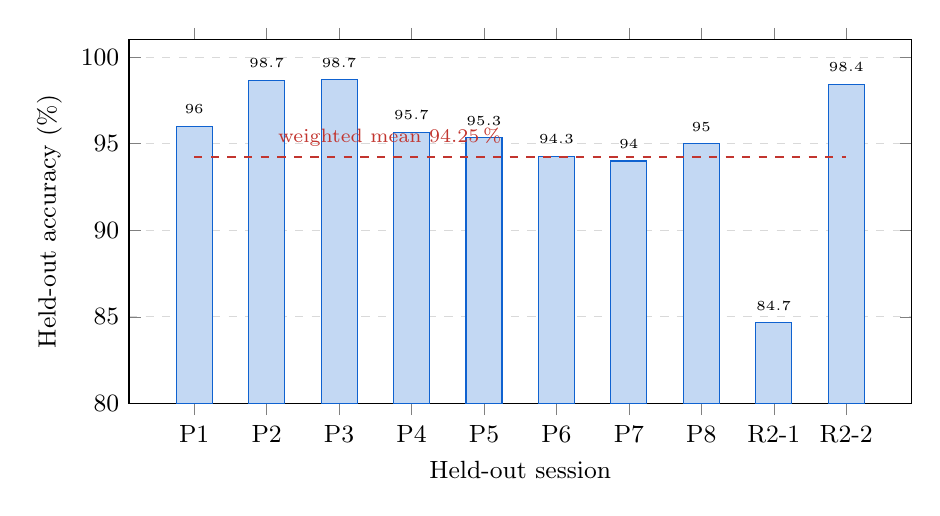
\begin{tikzpicture}
\begin{axis}[
    width=0.95\linewidth, height=6.2cm,
    ybar,
    bar width=13pt,
    ymin=80, ymax=101,
    ylabel={Held-out accuracy (\%)},
    xlabel={Held-out session},
    symbolic x coords={P1,P2,P3,P4,P5,P6,P7,P8,R2-1,R2-2},
    xtick=data,
    ymajorgrids=true,
    grid style={dashed, gray!30},
    nodes near coords,
    nodes near coords style={font=\tiny, /pgf/number format/fixed,
                             /pgf/number format/precision=1},
    every node near coord/.append style={yshift=1pt},
    tick label style={font=\small},
    label style={font=\small},
]
\addplot[draw=accent, fill=accent!25] coordinates {
  (P1,96.00) (P2,98.67) (P3,98.69) (P4,95.67) (P5,95.33)
  (P6,94.28) (P7,94.00) (P8,95.00) (R2-1,84.67) (R2-2,98.44)
};
\draw[dashed, thick, bad] (axis cs:P1,94.25) -- (axis cs:R2-2,94.25)
  node[pos=0.30, above, font=\scriptsize, bad] {weighted mean 94.25\,\%};
\end{axis}
\end{tikzpicture}
\caption{Accuracy on each held-out session. \code{P1}--\code{P8} are the room-1
sessions; \code{R2-1} and \code{R2-2} are the room-2 sessions. The spread is the
result, not the mean: a 94.25\,\% average contains a fold at 84.67\,\%.}
\label{fig:folds}
\end{figure}

\subsection{Interpretation}

The mean should not be reported alone. The distribution in
Figure~\ref{fig:folds} is bimodal in character: seven sessions fall between
94\,\% and 99\,\%, one falls to 84.67\,\%, and the difference between them is
not random. Section~\ref{sec:noise} shows that it tracks a measurable property
of the recording environment.

The cross-room figure deserves particular care. When a model trained only on
the eight room-1 sessions was scored on an untouched room-2 session, it
achieved 82.50\,\%. This is materially above chance and constitutes real
evidence that the representation transfers, but it is also clearly worse than
within-room performance. Once both room-2 sessions were included in training,
the ten-session leave-one-session-out figure recovered to 94.25\,\%. The honest
reading is that \textbf{a new room costs approximately 12 percentage points
until data from it is collected}.

%==============================================================================
\section{Environmental Dependence: the Noise Floor}
\label{sec:noise}
%==============================================================================

\subsection{Motivation}

Early in the project, variation in accuracy between sessions was treated as
model instability. It is not. It is a property of the recording environment,
and it can be measured directly and cheaply --- during the calibration period
that the system already performs.

\subsection{Definition}

The metric is the mean frame-to-frame amplitude change while the room is empty,
\emph{divided by} the mean amplitude:
\begin{equation}
  E = \frac{1}{T-1}\sum_{t=1}^{T-1}\frac{1}{K}\sum_{k=1}^{K}
      \bigl| a_k(t+1) - a_k(t) \bigr|,
  \qquad
  A = \frac{1}{|\mathcal{K}_{\mathrm{act}}|}\!\!\sum_{k \in \mathcal{K}_{\mathrm{act}}}\!\! \bar{a}_k,
  \qquad
  N = \frac{E}{A},
  \label{eq:noise}
\end{equation}
where $\mathcal{K}_{\mathrm{act}}$ is the set of active (non-guard-band)
subcarriers. $N$ is dimensionless: it expresses jitter as a \emph{fraction of
received signal} rather than in raw amplitude units.

\subsection{Why the division is necessary}

The first version of this metric used $E$ alone. That is adequate for watching
one board over time but is wrong for comparing two boards, and the error was
found by measurement rather than by reasoning. Two boards were placed at the
\emph{same} location and recorded simultaneously:

\begin{table}[H]
\centering
\caption{Two receivers at the same physical location. On the raw scale, node B
appears cleaner than node A. It is not.}
\label{tab:nodeab}
\begin{tabular}{@{}lrrrr@{}}
\toprule
\textbf{Board} & \textbf{RSSI (dBm)} & \textbf{Mean amplitude} & \textbf{Raw jitter $E$} & \textbf{Relative $N$} \\
\midrule
Node A & $-47.0$ & 32.1 & 1.63 & \textbf{0.051} \\
Node B & $-59.3$ & 16.6 & 1.17 & \textbf{0.071} \\
\bottomrule
\end{tabular}
\end{table}

\keyfinding{Node B receives 12\,dB less signal, so its amplitudes --- and hence
its raw frame-to-frame differences --- are proportionally smaller. On the raw
scale it therefore appears \emph{cleaner} than node A, while in fact it is
approximately \textbf{39\,\% noisier relative to what it receives}. Dividing by
amplitude makes the two comparable. This was a defect in the measurement
design, not in the system being measured.}

\subsection{Thresholds and per-session values}

The thresholds are read off the project's own ten sessions rather than chosen
by intuition: \emph{quiet} at $N \leq 0.06$, \emph{loud} at $N \geq 0.15$, and
\emph{moderate} between. Table~\ref{tab:noise} reports, for each session, the
noise floor, the ratio of mean moving energy to mean empty energy (the
``separation''), and the held-out accuracy.

\begin{table}[H]
\centering
\caption{Empty-room noise floor, class separation and held-out accuracy,
ordered by noise floor.}
\label{tab:noise}
\begin{tabular}{@{}lrrrl@{}}
\toprule
\textbf{Session} & \textbf{Noise floor $N$} & \textbf{Separation} & \textbf{Accuracy} & \textbf{Grade} \\
\midrule
\code{part\_1\_data}       & 0.0249 & 4.66$\times$ & 96.00\,\% & quiet \\
\code{part\_4\_data}       & 0.0258 & 3.80$\times$ & 95.67\,\% & quiet \\
\code{part\_2\_data}       & 0.0312 & 3.13$\times$ & 98.67\,\% & quiet \\
\code{part\_3\_data}       & 0.0357 & 2.88$\times$ & 98.69\,\% & quiet \\
\code{part\_5\_data}       & 0.0445 & 5.95$\times$ & 95.33\,\% & quiet \\
\code{part\_7\_data}       & 0.0996 & 1.36$\times$ & 94.00\,\% & moderate \\
\code{room2\_part\_2\_data}& 0.1375 & 1.89$\times$ & 98.44\,\% & moderate \\
\code{part\_8\_data}       & 0.2163 & 0.99$\times$ & 95.00\,\% & loud \\
\code{part\_6\_data}       & 0.2209 & 1.02$\times$ & 94.28\,\% & loud \\
\code{room2\_part\_1\_data}& 0.2209 & 1.02$\times$ & 84.67\,\% & loud \\
\bottomrule
\end{tabular}
\end{table}

\begin{figure}[H]
\centering
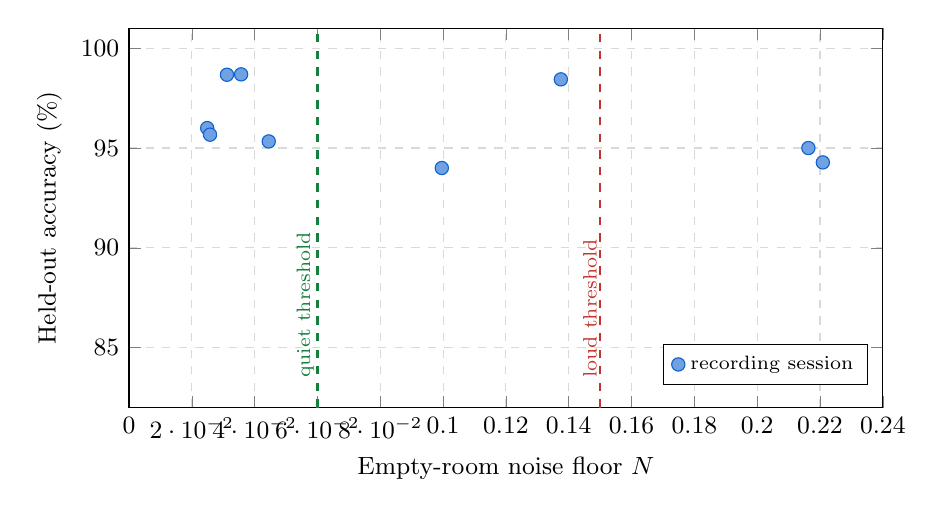
\begin{tikzpicture}
\begin{axis}[
    width=0.92\linewidth, height=6.4cm,
    xlabel={Empty-room noise floor $N$},
    ylabel={Held-out accuracy (\%)},
    xmin=0, xmax=0.24, ymin=82, ymax=101,
    ymajorgrids=true, xmajorgrids=true,
    grid style={dashed, gray!30},
    tick label style={font=\small},
    label style={font=\small},
    legend style={font=\scriptsize, at={(0.98,0.06)}, anchor=south east},
]
\addplot[only marks, mark=*, mark size=2.4pt, draw=accent, fill=accent!60]
  coordinates {
    (0.0249,96.00) (0.0258,95.67) (0.0312,98.67) (0.0357,98.69)
    (0.0445,95.33) (0.0996,94.00) (0.1375,98.44) (0.2163,95.00)
    (0.2209,94.28) (0.2209,84.67)
  };
\addlegendentry{recording session}
\draw[dashed, good, thick] (axis cs:0.06,82) -- (axis cs:0.06,101);
\draw[dashed, bad, thick]  (axis cs:0.15,82) -- (axis cs:0.15,101);
\node[font=\scriptsize, good, anchor=south west, rotate=90] at (axis cs:0.062,83) {quiet threshold};
\node[font=\scriptsize, bad,  anchor=south west, rotate=90] at (axis cs:0.152,83) {loud threshold};
\end{axis}
\end{tikzpicture}
\caption{Held-out accuracy against empty-room noise floor. The relationship is
real in aggregate but weak per session: two sessions at $N \approx 0.22$ scored
94.28\,\% and 84.67\,\%.}
\label{fig:noise}
\end{figure}

\subsection{What the metric does and does not predict}

Above approximately $N = 0.15$ the aggregate motion signal has essentially
vanished: mean empty energy and mean moving energy come within about 2\,\% of
each other, and the classes are separable only through finer per-subcarrier
structure. This is visible in the separation column of Table~\ref{tab:noise},
which falls from 4.66$\times$ to almost exactly 1.

It is nonetheless important not to overstate the metric:

\keyfinding{A loud noise floor is a \textbf{risk indicator, not a forecast}.
\code{part\_6\_data} and \code{part\_8\_data} sit at the very top of the scale
and still scored 94--95\,\%, while \roomA{} at a near-identical floor scored
84.67\,\%. Grouped, the effect is real --- 87.8\,\% within loud sessions against
94.1\,\% within quiet ones --- but it does not predict the outcome of any
individual session.}

\noindent
The practical value of the metric is therefore diagnostic rather than
predictive: it tells the operator which regime the system is currently
operating in, so that a period of unreliable behaviour can be attributed to the
environment rather than misdiagnosed as a broken model. The live system reports
the grade after every calibration.

Common causes of a high floor observed during the project were Wi-Fi congestion
on the operating channel, a fan or air-conditioning unit running, USB\,3.0 ports
and cables radiating in the 2.4\,GHz band, and weak reception causing
quantisation noise --- CSI arrives as signed 8-bit values, so a weak signal sits
near $\pm 4$ counts where one quantisation step is a large fraction of the
value, and the amplitude jitters even with nothing moving.

%==============================================================================
\section{Live Inference System}
%==============================================================================

Offline accuracy does not by itself produce a usable system. Several mechanisms
exist purely to make the live behaviour trustworthy.

\subsection{Prediction smoothing}

The classifier emits one prediction per 0.75\,s window. Displaying that
directly makes the output flicker, because a single unlucky window can flip the
state. A hysteresis stage therefore requires a majority of the last five raw
predictions to agree before the confirmed state changes. The user interface
distinguishes the raw per-window prediction from the confirmed state and
reports the vote fraction behind the latter.

\subsection{Rolling recalibration}

The live system mirrors the per-block recalibration used during training. Once
the system has been confirmed empty for a sustained period, it refreshes its
baseline rather than comparing against the startup snapshot indefinitely.

A first implementation of this drifted into predicting MOVING in an empty room,
sometimes within a single session. Two safety mechanisms were added, each
addressing a distinct failure:

\begin{enumerate}[leftmargin=1.6em, itemsep=3pt]
  \item \textbf{Blend, do not replace.} A ten-second sample is a noisy estimate
        of the true noise floor and can land quieter than typical by chance.
        Replacing the baseline outright with each such sample lets one unlucky
        quiet window ratchet sensitivity upward with nothing pulling it back.
        A weighted step toward the fresh sample ($\alpha = 0.3$) still tracks
        genuine drift over many cycles, but no single sample can dominate.
  \item \textbf{Floor against the startup baseline.} No blended standard
        deviation may fall below 60\,\% of what the original, deliberate
        ``leave the room'' calibration measured. That calibration is a trusted
        reference; nothing is permitted to make the system \emph{more}
        sensitive than it ever was, only less, so as to absorb a genuinely
        louder environment such as an air conditioner starting.
\end{enumerate}

\noindent
The rolling calibrator never observes frames while MOVING is confirmed, and its
buffer resets the moment motion is confirmed, so a burst of activity cannot
contaminate the baseline.

\subsection{Two-node operation and OR fusion}

A single link is most sensitive to movement near the direct path between the
receiver and the access point; movement well off that axis perturbs it more
weakly. This is a property of single-link CSI sensing rather than a defect.

Running two physically separated receivers gives two different direct paths, so
a person in one node's weak region is frequently in the other's strong region.
The two pipelines are entirely independent --- separate serial ports, baselines,
windows and smoothers --- and are combined with OR logic: if either node
confirms MOVING, the room is reported as MOVING. This requires no additional
training data and no clock synchronisation between the boards.

The cost of OR fusion is that a single node producing false alarms causes the
whole system to produce them. Section~\ref{sec:negative} describes the
measurement that led to a manual rather than automatic remedy.

\subsection{Degradation semantics}

The following rule is enforced throughout the live system and the dashboard:

\keyfinding{A node that is offline or muted is excluded from the vote entirely.
If \emph{no} node is voting, the result is \emph{unknown} --- never EMPTY. An
empty room is never inferred from the absence of working sensors.}

\noindent
This is not a cosmetic choice. An earlier version left a dead node's state at
``unknown'' while still requiring all nodes to agree before reporting EMPTY,
with the result that a single misconfigured serial port made it impossible for
the system ever to return to EMPTY: the room would correctly report MOVING and
then remain stuck indefinitely.

Similarly, a sustained change in subcarrier count --- the access point
renegotiating its channel width mid-session --- previously caused every
subsequent frame to fail a length check and be discarded, so the affected node
went permanently and silently dead. The system now re-latches to the new count
after twenty sustained frames, restarts calibration, and warns that predictions
are disabled for that node until the width matches.

\subsection{Operator interface}

The system is monitored through a browser dashboard. A single self-contained
HTML file serves both deployments: opened from disk it connects to the host
process, while served over HTTP it connects back to whichever host served it,
which is how the same file is embedded in the firmware and served by the board
itself. It has no external dependencies of any kind --- no remote fonts,
scripts or images --- because a single outbound request would break the
standalone deployment.

The interface presents, in descending order of prominence: the confirmed
combined state; the vote fraction behind it; each node's individual state,
received signal strength and motion energy; a \emph{waterfall} visualisation of
per-subcarrier amplitude over time; the motion-energy trace; session
statistics; and the calibration and noise-floor readout of
Section~\ref{sec:noise}.

The waterfall is the most directly interpretable artefact the project
produces. Amplitude is mapped to colour with subcarrier index on one axis and
time on the other, so a still room renders as smooth horizontal banding --- each
subcarrier holding its own steady value --- and a person moving visibly breaks
that banding into churn. It makes the physical claim of
Section~\ref{sec:features} legible without reference to any model output.

Three interface principles follow directly from the honesty requirement stated
earlier and are worth recording, since they are design decisions rather than
decoration:

\begin{enumerate}[leftmargin=1.6em, itemsep=3pt]
  \item \textbf{Transitional states must not resemble readings.} Warming up and
        calibrating are rendered at body scale with outline iconography and a
        provisional treatment, while confirmed EMPTY and MOVING are rendered at
        display scale with solid iconography. A viewer glancing at the screen
        cannot mistake ``I do not know yet'' for ``the room is empty''.
  \item \textbf{The three non-contributing conditions are visually distinct.}
        \emph{Offline} is a fault, \emph{muted} is an operator decision, and
        \emph{warming up} is simply not knowing yet. Collapsing them into one
        appearance would imply that a dead sensor is about to recover.
  \item \textbf{Explanations exclude what is excluded.} When the interface
        states that a result was confirmed by some number of nodes, offline and
        muted nodes are omitted from that count, so the reported coverage never
        exceeds the coverage that actually exists.
\end{enumerate}

\noindent
The noise floor is presented as a meter with marks at the two graded
thresholds, rather than as a bare number, so that an operator can judge the
environment without consulting documentation; the exact value remains on screen
for technical use. Faults, node degradations and occupancy alerts are presented
as a stack of individually timestamped conditions keyed by node, so that a
condition affecting one node can neither overwrite nor silently resolve a
condition affecting another.

%==============================================================================
\section{Recurring Failures Fixed at Source}
\label{sec:recurring}
%==============================================================================

Two failures each recurred three times during the project. In both cases every
earlier remedy consisted of adjusting a value that would inevitably go stale
again. They are recorded here because the pattern --- distinguishing a fix from
a workaround --- is the most transferable lesson in the work.

\begin{table}[H]
\centering
\caption{Two recurring failures and their eventual root-cause remedies.}
\begin{tabularx}{\linewidth}{@{}lXX@{}}
\toprule
\textbf{Failure} & \textbf{Previous remedy} & \textbf{Root-cause fix} \\
\midrule
192 subcarriers instead of 128 &
``Change the access point's channel width'' --- not even available on a mobile
hotspot &
The station itself advertises 20\,MHz only, so the access point cannot raise the
link width regardless of its own configuration \\
\addlinespace
No CSI produced at all &
Correct the hardcoded router address in the firmware &
Take the ping target from the board's own DHCP lease, which is correct by
construction \\
\bottomrule
\end{tabularx}
\end{table}

\noindent
The second case is worth expanding. CSI exists only when packets arrive, and the
firmware manufactures that traffic by pinging the router. When the ping target
was a compiled-in constant, the board would boot, join the network, log ``CSI
enabled'' and then emit nothing at all --- a failure that presents identically
to a broken sensor. The mobile hotspot used during development was observed to
reassign its subnet from \code{10.170.51.x} to \code{172.22.34.x} to
\code{192.168.43.x} within a single session. Deriving the target from the DHCP
lease removes the possibility of the mismatch entirely.

%==============================================================================
\section{Embedded Deployment}
\label{sec:embedded}
%==============================================================================

\subsection{Scope}

Training remains on the host; only \emph{inference} was moved to the device.
This is the conventional division for embedded machine learning and avoids
pretending that the microcontroller can retrain itself. The workflow is:
record, train on the host, export, flash.

\subsection{Feasibility, measured before implementation}

\begin{itemize}[leftmargin=1.4em, itemsep=3pt]
  \item The full 200-tree forest packs to approximately \textbf{430\,kB} of C,
        which is about 2.7\,\% of the available flash. There was consequently no
        reason to prune the model, and the board runs \emph{exactly} the forest
        that was validated offline --- so every accuracy figure in
        Section~\ref{sec:results} continues to describe the hardware. For
        contrast, reducing to 25 trees would have cost 0.67 percentage points
        (93.58\,\% against 94.25\,\%) for an eightfold space saving.
  \item Runtime memory is modest: approximately 6\,kB for the window buffer,
        baseline and feature vector, with about 107\,kB of static scratch
        buffers.
  \item \textbf{Single-precision arithmetic was the principal risk and it did
        not materialise.} Across all 3302 recorded windows, evaluating in
        \code{float32} rather than \code{float64} changed \textbf{zero}
        predictions, despite 2.7\,\% of windows lying within 0.10 of the
        decision boundary. Relative feature drift was of order $10^{-8}$, far
        below the resolution of any tree threshold.
\end{itemize}

\subsection{Export format}

The exporter emits four parallel arrays rather than an array of structures. A
structure of \code{\{int16, float, int16, int16\}} occupies ten bytes of data
that the compiler pads to twelve for float alignment, wasting approximately
85\,kB across 44\,000 nodes; parallel arrays keep it at exactly ten bytes per
node.

One subtlety is essential for correctness. A Random Forest's
\code{predict\_proba} averages each tree's \emph{probability distribution} ---
the normalised class counts at the reached leaf --- and then takes the
arg\-max. It does \emph{not} take a majority vote of hard per-tree labels, and
the two differ whenever trees are impure. Leaves therefore store a probability
rather than a class. With two classes only $p_1$ need be stored. Furthermore,
the reference implementation's arg\-max returns the \emph{first} maximum, so an
exact tie at $0.5$ resolves to class 0; the generated C uses a strict
$p_1 > 0.5$ comparison to reproduce this exactly.

\subsection{Verification}

\begin{table}[H]
\centering
\caption{Verification of the embedded port.}
\begin{tabularx}{\linewidth}{@{}Xr@{}}
\toprule
\textbf{Check} & \textbf{Result} \\
\midrule
Generated C simulation against the reference implementation, all windows & \textbf{3302 / 3302} identical \\
On-device boot self-test, predictions & \textbf{12 / 12} identical \\
On-device boot self-test, features within tolerance & \textbf{266 / 266} \\
\code{float32} against \code{float64}, all windows & \textbf{0} prediction changes \\
Serial \code{CSI\_AMP} stream unchanged by the addition & verified by diff \\
\bottomrule
\end{tabularx}
\end{table}

\noindent
Because no host C compiler was available, the self-test embeds real recorded
frames together with the host's answers and recomputes the baseline, all 266
features and the prediction from scratch at boot. This turned out to be the
stronger choice: it exercises the actual floating-point unit and the actual
cross-compiler, which is precisely where a port of this kind fails.

One self-test vector is deliberately a window that the model classifies
\emph{incorrectly}, and the device reproduces the same incorrect answer. This is
the point: the test verifies fidelity to the reference implementation, not
agreement with ground truth.

\subsection{A bug findable only on hardware}

After the parity self-test had already passed, the firmware entered a boot
loop. The cause was a main-task stack overflow: a single feature computation
required approximately 3.4\,kB of stack against the real-time operating
system's 3584-byte default. The scratch arrays were made static and the stack
was enlarged.

\keyfinding{A host-compiled unit test would have passed this without
difficulty, because desktop stacks are measured in megabytes. Some categories
of embedded defect are only reachable on the target.}

\subsection{Standalone operation}

The board additionally runs the detection state machine --- warm-up, then a
100-frame calibration, then continuous classification --- and serves the
project's own dashboard over HTTP and WebSocket, so a phone on the same network
can view the system with no computer involved.

The addition is strictly \emph{additive}: the firmware still prints its
\code{CSI\_AMP} line first and unchanged, before any inference runs, so the
host pipeline continues to work identically with the new firmware installed.
Standalone mode is single-node, as peer-to-peer communication between boards was
not implemented, and it cannot raise alerts.

%==============================================================================
\section{Alerting}
%==============================================================================

The host application can invoke an action --- an HTTP webhook, an email, or an
arbitrary command --- when the room has been continuously occupied. The design
question is how long to wait before acting, and it was settled by measurement
rather than preference.

Per-window false alarms run at approximately 11\,\% in a noisy room. Requiring
several \emph{consecutive} seconds of confirmed MOVING collapses this to
roughly one spurious alert per recording session, and to none at all across the
quiet sessions. The hold does most of the work of making an alert trustworthy;
a five-second threshold was adopted, with a sixty-second cooldown so that one
person moving about does not generate a continuous stream of notifications.

\keyfinding{The evidence behind this threshold is thin and should be described
as such. It was measured over only about \textbf{21 minutes} of empty-room
recording, which bounds the false-alert rate loosely rather than establishing
it. In a room with a noise floor above approximately 0.15, spurious alerts
several times an hour should be expected.}

\noindent
A security detail worth recording: the mail password is read from an
environment variable and is deliberately \emph{not} accepted as a command-line
argument, because arguments are visible to every other process on the machine
and are written into shell history. A unit test asserts that no such flag
exists.

%==============================================================================
\section{Negative Results}
\label{sec:negative}
%==============================================================================

Three results are reported here that did not lead to a change in the system.
They are included because a project that reports only its successes provides no
evidence that its methods are capable of detecting failure.

\subsection{A refuted hypothesis}

It was predicted that the two aggregate motion-energy features were redundant
given the per-subcarrier features, and that removing them would improve
cross-room transfer. Six ablation experiments were run. Removing them made
performance \emph{worse}, from 94.25\,\% to 94.00\,\%. The hypothesis was
abandoned and the features retained.

\subsection{A proposed feature that failed its acceptance test}

Because nodes are combined with OR logic, one node producing false alarms
causes the entire system to produce them. An automatic gating mechanism was
proposed, which would use the measured noise floor to withdraw an unreliable
node's vote. It was tested before being built.

\begin{itemize}[leftmargin=1.4em, itemsep=2pt]
  \item Increasing the smoothing window from five to nine moved the false-alarm
        rate from 12.6\,\% to 12.7\,\% --- no useful effect.
  \item The noise floor correlates with false-alarm rate at only $-0.50$.
  \item Decisively: two sessions with almost identical noise floors, 0.216 and
        0.221, had false-alarm rates of \textbf{0.7\,\%} and \textbf{26.3\,\%}.
\end{itemize}

\noindent
The noise reading therefore cannot identify which node will misbehave, and an
automatic mechanism would have silenced sound nodes as often as faulty ones. A
\emph{manual} mute control was implemented instead: the operator can see which
node is misbehaving and withdraw its vote without restarting anything, while
the node continues to stream and remains fully visible.

\subsection{A silent configuration defect}

Running the training script with no arguments had, for a period, retrained on
four sessions at a 2.0-second window --- values left over from early
development --- silently overwriting the deployed model with a weaker one.
Separately, four analysis scripts had each drifted to a \emph{different} stale
session list, so each was reporting results about a configuration that was not
deployed.

The remedy was to define the deployed configuration once and import it
everywhere, and to add tests asserting that no analysis script defines its own
session list and that the default window matches the model actually on disk.

%==============================================================================
\section{Testing and Robustness Engineering}
%==============================================================================

The project includes \textbf{72 automated tests}, none of which require
hardware. Their focus is deliberate and worth stating, because it differs from
the usual emphasis in a machine learning project:

\keyfinding{The tests principally pin \emph{live-system failure modes} rather
than model accuracy --- malformed serial lines, a node going offline, the
access point changing channel width mid-run. Every defect this project
encountered twice was a failure-mode defect, not a mathematical one.}

\begin{table}[H]
\centering
\caption{Coverage of the automated test suite.}
\begin{tabularx}{\linewidth}{@{}lX@{}}
\toprule
\textbf{Area} & \textbf{Examples} \\
\midrule
Parsing & valid lines, leading noise, malformed input, and verification that the
declared subcarrier count matches the number of amplitudes actually received \\
Node fusion & seventeen truth-table cases, including that an entirely
muted or offline system reports \emph{unknown} and never EMPTY \\
Calibration & the dead-subcarrier ratio blow-up is prevented; the rolling
calibrator ignores moving frames; the floor prevents a sensitivity ratchet \\
Noise floor & the ten real sessions are graded correctly; the metric is
scale-free across receivers of differing sensitivity \\
Alerting & the hold is respected; brief bursts are ignored; the cooldown
behaves; alerts never fire on an unknown state \\
Security & the mail password must come from the environment; no password
command-line flag may exist \\
Configuration drift & analysis scripts must not hardcode session lists; the
default window must match the deployed model \\
\bottomrule
\end{tabularx}
\end{table}

\noindent
A related discipline was adopted for documentation: every reported figure is
regenerated by running the corresponding script, and no accuracy number is
written by hand into any document.

%==============================================================================
\section{Limitations}
\label{sec:limitations}
%==============================================================================

\begin{table}[H]
\centering
\caption{Honest statement of what has and has not been established.}
\label{tab:limits}
\begin{tabularx}{\linewidth}{@{}lX@{}}
\toprule
\textbf{Dimension} & \textbf{Status} \\
\midrule
\textbf{People} & \textbf{One.} All training data is a single person's
movement. A second person has never been tested. This is the largest
outstanding gap and the most likely source of overestimated performance. \\
Movement styles & One --- that person's ordinary walking. \\
Rooms & Two. Cross-room transfer measured once, at 82.50\,\%. \\
Receivers & One board model, two units. \\
Access points & Not systematically varied. \\
Held-out data & \textbf{No permanently held-out set.} Every session
contributes to the final model; all held-out figures come from rotating
exclusion. \\
Motionless occupant & Not detectable; classified as EMPTY. \\
Multiple occupants & Not distinguished. \\
Position & Not measured. A two-zone classifier exists in the codebase but
\textbf{no zone data has ever been recorded}, so it is entirely unproven. \\
Through-wall operation & Untested and not claimed. \\
Unattended operation & Not burn-tested over long periods. \\
Safety-critical use & Explicitly unsuitable. \\
\bottomrule
\end{tabularx}
\end{table}

\subsection{On the absence of a permanent test set}

This deserves an explicit paragraph rather than a table row. Because every
session is eventually folded into training, the reported figures are
out-of-fold estimates rather than measurements on data the model has never
influenced. Leave-one-session-out is a sound estimator and the
\code{evaluate\_holdout.py} tool provides genuine single-shot held-out figures
on demand, but a permanently reserved session --- ideally recorded in a third
room, by a second person --- would be a stronger basis for the headline claim.

\subsection{On position estimation}

The codebase contains a two-zone classifier which runs only when motion has
already been confirmed and which leaves the binary model untouched. It is
reported here as \emph{unproven}, not as a result: no session on disk contains a
zone label. The script deliberately refuses to report an accuracy figure if any
session contains only one zone, because a model can then achieve near-perfect
scores by learning which \emph{session} it is looking at while knowing nothing
about position. A zone model would additionally be room-specific, since it must
rely on exactly the index-based features that do not transfer between rooms.

%==============================================================================
\section{Conclusions and Future Work}
%==============================================================================

\subsection{Conclusions}

A device-free motion detection system was built on commodity hardware and
evaluated with session-level cross-validation, reaching 94.25\,\% per-window
accuracy across ten recordings in two rooms. The same model was shown to run on
the microcontroller itself with exact numerical parity against the host
implementation, enabling operation with no computer attached.

The most defensible conclusion of the work, however, is methodological rather
than numerical:

\keyfinding{A single accuracy figure is the wrong way to characterise a Wi-Fi
sensing system. Performance is governed by a measurable property of the
environment --- the empty-room noise floor --- which varied by roughly a factor
of nine across this project's own recordings and which corresponded to accuracy
between 84.67\,\% and 98.69\,\%. A system of this kind should measure that
property and report which regime it is operating in, rather than presenting a
single number and degrading silently when conditions change.}

\subsection{Future work}

In descending order of expected value:

\begin{enumerate}[leftmargin=1.6em, itemsep=3pt]
  \item \textbf{A second person.} The single largest untested assumption. All
        current data reflects one individual's height, gait and movement style.
  \item \textbf{A third room}, to convert a single cross-room data point into a
        trend.
  \item \textbf{A permanently held-out session}, recorded in a new room by a new
        person and never used for training.
  \item \textbf{Zone data}, recorded with both zones alternating within every
        session across at least two days, and evaluated against the existing
        decision gate.
  \item \textbf{Peer-to-peer communication between boards}, so that two-node OR
        fusion works in standalone mode without a host.
  \item \textbf{Long unattended operation}, to characterise drift and
        false-alarm rates over days rather than minutes.
\end{enumerate}

%==============================================================================
\appendix
\section{Reproducing the Results}
%==============================================================================

All figures in Section~\ref{sec:results} are regenerated by the following
commands, executed from the repository root.

\begin{lstlisting}[language=bash, caption={Reproduction commands.}]
# environment
python -m venv .venv
python -m pip install -r requirements.txt

# reproduces the deployed model and every headline number
python train_model.py

# single-shot held-out evaluation on a named session
python evaluate_holdout.py --test room2_part_1_data

# comparison of six model families under identical validation
python compare_models.py

# multi-page PDF report: confusion matrix, feature correlation,
# two overfitting diagnostics and a health summary
python model_evaluation.py

# the automated test suite (72 tests, no hardware required)
python -m pytest tests/
\end{lstlisting}

\noindent
\textbf{Note.} \code{train\_model.py} overwrites \code{csi\_model.joblib} by
default. Use \code{--model-out} to write elsewhere when experimenting.

%==============================================================================
\section{Principal Source Files}
%==============================================================================

\begin{table}[H]
\centering
\caption{Principal components of the implementation.}
\begin{tabularx}{\linewidth}{@{}lX@{}}
\toprule
\textbf{File} & \textbf{Responsibility} \\
\midrule
\code{csi\_common.py} & \textbf{Single source of truth} for parsing, feature
extraction, calibration and smoothing. Imported by the training and both live
paths so that offline and online behaviour cannot diverge. \\
\code{csi\_label\_collector.py} & Auto-cycling data collection protocol. \\
\code{train\_model.py} & Dataset construction, leave-one-session-out validation
and model persistence. \\
\code{csi\_live\_server.py} & Live inference, one or two nodes, OR fusion,
degradation handling and alerting. \\
\code{csi\_dashboard.html} & Self-contained browser interface; also embedded
into the firmware and served by the board. \\
\code{diagnose\_nodes.py} & Distinguishes a noisy environment from a poorly
receiving board. \\
\code{export\_model\_c.py} & Exports the forest to C with verification against
the reference implementation. \\
\code{firmware/main/csi\_node.c} & CSI capture, ping trigger, serial output. \\
\code{firmware/main/csi\_features.c} & The 266 features reimplemented in C. \\
\code{tests/test\_pipeline.py} & The 72-test suite. \\
\code{docs/PROJECT\_HISTORY.md} & Full chronological development record. \\
\bottomrule
\end{tabularx}
\end{table}

%==============================================================================
\section{Optional Figures}
%==============================================================================

The document deliberately contains no external image files so that it always
compiles. To add screenshots --- the dashboard waterfall is the most
persuasive single image in the project, since stable horizontal banding
visibly breaks up when a person moves --- place the image file alongside this
\code{.tex} file and uncomment the block below.

\begin{lstlisting}[caption={Template for adding a screenshot.}]
% \begin{figure}[H]
%   \centering
%   \includegraphics[width=0.9\linewidth]{dashboard_moving.png}
%   \caption{Live dashboard while motion is confirmed. The waterfall shows
%            stable per-subcarrier banding breaking up as a person moves.}
%   \label{fig:dashboard}
% \end{figure}
\end{lstlisting}

%==============================================================================
\section*{References}
\addcontentsline{toc}{section}{References}
%==============================================================================

\noindent
The following are the primary technical resources relied on during
implementation. \textbf{Add your own academic citations here as required by your
institution} --- in particular, survey literature on Wi-Fi sensing and on CSI
phase sanitisation, neither of which is cited above because neither was used.

\begin{enumerate}[leftmargin=1.6em, itemsep=3pt]
  \item Espressif Systems, \textit{ESP-IDF Programming Guide}, v6.0.
        \url{https://docs.espressif.com/projects/esp-idf/en/stable/esp32s3/}
  \item scikit-learn developers, \textit{scikit-learn: Machine Learning in
        Python}. \url{https://scikit-learn.org/}
  \item Project source code, datasets and full development history.
        \url{https://github.com/IALR/csi-motion-detection}
\end{enumerate}

\end{document}
